% !TEX root = LF-IMAPol.tex

\chapter{Introduction}\label{chap:Introduction}

\section{Our object of study: lexical functions}\label{sec:aboutWhat}

This book is about \notion{lexical functions}\index[notion]{lexical function}. Therefore, our very first task is to explain -- at least, approximately, in simple terms and with the help of most trivial examples -- what lexical functions are. Let's do it!

Consider the phrases in \Next and \NNext:\footnote{As is customary, we use the asterisk ``*'' in front of an expression to indicate that this expression is ungrammatical. Let it be emphasized that for an expression to be ungrammatical does not imply that it cannot be found in speech. For instance, at the time of writing, the one-billion-word Corpus of Contemporary American English \parencite{Davies2008} contained 1,676 occurrences of \textit{pay tribute} and 13 occurrences of the ungrammatical phrase *\textit{give tribute} (for all inflected forms of these phrases). Additionally, the acceptability of word combinations can fluctuate significantly due to geographical variation. We are grateful to Alastair Butler for the suggestion to use \ref{ex:payTribute} and \ref{ex:giveRecognition} as illustrations.}\index[notion]{ungrammaticality}\index[notion]{COCA corpus}

\begingroup
\small

\ex.\label{ex:payTribute} \a. \emph{pay} tribute \lfgp{to someone}
     \b. *\emph{give} tribute \lfgp{to someone}

\ex.\label{ex:giveRecognition} \a. \emph{give} recognition \lfgp{to someone}
     \b. *\emph{pay} recognition \lfgp{to someone}\hspace{25pt}

\endgroup

The verbs \textit{pay} and \textit{give}, used in \LLast[a] and \Last[a] with the nouns \textit{tribute} and \textit{recognition}, respec­tively, are not interchangeable in spite of the following facts:

\begin{itemize}

\item The two nouns are semantically close.

\item The two verbs are, so to speak, pure verbalizers\index[notion]{verbalizer} of their nominal objects: they express a very general, impoverished meaning, approximately `do', and add no semantic content to the nouns.

\end{itemize}

These verbs are empty of meaning in the given contexts to such an extent that \textit{pay tribute} is semantically reducible to a hypothetical verb *\textit{to tribute} \lfgp{\textit{someone}}, and \textit{give recognition}, to the verb \textit{to recognize} \lfgp{\textit{someone} (\textit{during a ceremony})}. For this reason, verbs such as \textit{pay} and \textit{give} are called \emph{support}, or \emph{light}, verbs\index[notion]{support verb}\index[notion]{verb!support \tld} (see \chapref{chap:syntLFs}, \sectref{sec:verbeSupport}).

The choice of the appropriate support verb by the Speaker\index[notion]{Speaker, the} is, as one sees in \ref{ex:payTribute} and \ref{ex:giveRecognition}, contingent upon a specific nomin­al lexeme -- the direct object of this verb: the meaning `do' is ex­pressed by the verb \textit{pay} if you `do' \textit{tribute}, but by the verb \textit{give} if you `do' \textit{recognition}. In other words, the meaning `do' is expressed not freely\index[notion]{meaning!free \tld}, that is, not by any convenient verb the Speaker is able to think of. It is expressed in a constrained way\index[notion]{meaning!constrained \tld}: by the verb that the noun imposes. To borrow from the language of mathematics\index[notion]{mathematical function}, the meaning `do' is expressed \emph{as function of} the direct object of the corresponding verb. This is where the noun \textit{function} in the term \textit{lexical function} comes from. The reason for the adjective \textit{lexical} is obvious: such functions apply to lexical units\index[notion]{lexical unit} and return lexical entities\index[notion]{lexical entity} -- on the notion of lexical entity, see \sectref{sec:lexicalNotions} (p.\thinspace\pageref{def:lexicalEntity}).

\begin{soundbox}{Syntagmatic lexical function}
What is illustrated in \ref{ex:payTribute} and \ref{ex:giveRecognition} is a \emph{syntagmatic} lexical function\index[notion]{lexical function!syntagmatic \tld}\index[notion]{syntagmatic!\tld\ lexical function} called \lf{Oper\tsub{1}}\index[lf]{Operi@\lf{Oper\tsub{i}}!\lf{Oper\tsub{1}}} (see \chapref{chap:syntLFs}, [\ref{lf:Oper-i}], p.\thinspace\pageref{lf:Oper-i}), which describes a particular pattern of constrained lexical unit combinations -- that is, a particular type of a two-component phrase where one lexical unit, freely selected by the Speaker, determines the selection of the other lexical unit. In this specific case, borrowing again from mathematical formalization, we write:

\phantom{.}
\begingroup
\small

\ex.[] \setlength{\tabcolsep}{2pt}\begin{tabular}[t]{ l c >{\raggedright\arraybackslash}p{6cm} }
\lfappl{Oper\tsub{1}}{\textit{tribute}} & = & \textit{pay} \lfgp{\textit{tribute}} \\
\lfappl{Oper\tsub{1}}{\textit{recognition}} & = & \textit{give} \lfgp{\textit{recognition}} \\
\end{tabular}

\endgroup

Constrained lexical combinations described by syntagmatic lexical functions are termed \emph{collocations} (see \chapref{chap:NotionLF}, \sectref{sec:classeFLSyntagmatiques}). They are extremely varied -- support-verb constructions (presented above), realization-verb constructions (\textit{pay a debt}, \textit{satisfy a desire}, \textit{ring a bell}), \mbox{(de-)intensifying} modifier constructions (\textit{generous}\slashs\textit{meager salary}, \textit{remember clearly}\slashs\textit{vaguely}), etc. -- and their description requires a wide range of syntagmatic lexical functions.
\end{soundbox}

\largerpage[-1]
Lexical functions are not limited to constrained combinations of \emph{lexical units} within \emph{phrases}: they similarly deal with constrained combinations of \emph{morphemes}\index[notion]{morpheme} within \emph{wordforms}\index[notion]{wordform}. For instance, in English, the derivational means\index[notion]{derivative!morphological \tld} used to produce from a verb V the noun that means `person who does V' is contingent upon V, as illustrated in \Next:

\begingroup
\small
 
 \ex.\label{ex:S1Derivations} \begingroup\setlength{\tabcolsep}{2pt}
\begin{tabular}[t]{ l c l c >{\raggedright\arraybackslash}p{5cm} }
\textit{teach} & $\Rightarrow$ & \textit{teacher} & : & \textbf{-er} suffixation \\
\textit{represent} \lfgp{\textit{a social group}} & $\Rightarrow$ & \textit{representative}\tsub{(N)} & : & \textbf{-(at)ive} suffixation \\
\textit{chair}\tsub{(V)} \lfgp{\textit{a meeting}} & $\Rightarrow$ & \textit{chairperson} & : & compounding \\
\textit{guide}\tsub{(V)} & $\Rightarrow$ & \textit{guide}\tsub{(N)} & : & V\thinspace$\Rightarrow$\thinspace{}N conversion \\
\textit{steal}\tsub{(V)} & $\Rightarrow$ & \textit{thief} & : & suppletive form \\
\end{tabular}\endgroup

\endgroup\index[notion]{suffixation}\index[notion]{compounding}\index[notion]{conversion, morphological}\index[notion]{suppletion}

In parallel with what has been said about the meaning `do' for our first set of illustrations, we say that the meaning `person who does [V]' is expressed as function of the verb V in order to return the corresponding noun.

\begin{soundbox}{Paradigmatic lexical function}
The constrained combinations of morphemes\index[notion]{morpheme} illustrated in \ref{ex:S1Derivations} are also representable by means of a lexical function; in this case, a \emph{paradigmatic} lexical function\index[notion]{lexical function!paradigmatic \tld}\index[notion]{paradigmatic!\tld\ lexical function} called \lf{S\tsub{1}}\index[lf]{Si@\lf{S\tsub{i}}!\lf{S\tsub{1}}} (see \chapref{chap:paraLFs}, [\ref{lf:S-i}], p.\thinspace\pageref{lf:S-i}). Accordingly, we write:

\phantom{.}
\begingroup
\small

\ex.[] \setlength{\tabcolsep}{2pt}\begin{tabular}[t]{ l c >{\raggedright\arraybackslash}p{8cm} }
\lfappl{S\tsub{1}}{\textit{teach}} & = & \textit{teacher} \\
\lfappl{S\tsub{1}}{\textit{represent}} & = & \textit{representative}\tsub{(N)} \\
\lfappl{S\tsub{1}}{\textit{chair}\tsub{(V)}} & = & \textit{chairperson} \\
\lfappl{S\tsub{1}}{\textit{guide}\tsub{(V)}} & = & \textit{guide}\tsub{(N)} \\
\lfappl{S\tsub{1}}{\textit{steal}\tsub{(V)}} & = & \textit{thief} \\
\end{tabular}

\endgroup

\noindent
\remark{Notation.}As can be seen, we indicate in subscript the part of speech of a lexical unit if it has a homonym of a different part of speech.
\end{soundbox}

Summing up, lexical functions are a formal tool designed to describe specific patterns of constrained combinations of linguistic signs\index[notion]{linguistic sign} -- of lexical units as well as of morphemes\index[notion]{morpheme}.\footnote{The morphemes in question are mostly derivational morphemes, that is, morphemes whose meanings are fairly close to lexical meanings.} As such, lexical functions account for an important part of natural languages' phraseology\index[notion]{phraseology}:\footnote{On the notions of phraseme and phraseology, see \sectref{sec:lexicalNotions}, p.\thinspace\pageref{sec:lexicalNotions}.} lexical as well as morphological phraseology\index[notion]{phraseology!lexical \tld}\index[notion]{phraseology!morphological \tld} \parencite{Melcuk2021b}.\phantomsection\label{txt:LFsAndPhraseology}

The set of lexical functions is organized around a rigorously structured system of \emph{simple standard} lexical functions\index[notion]{lexical function!standard \tld}\index[notion]{system of standard LFs}\index[notion]{lexical function!system of standard \tlds}, whose number is under 70 (see \chapref{chap:NotionLF}, p.\thinspace\pageref{tab:systFL}). One of their defining properties is that they are language-universal\index[notion]{universal|see{language-universal}}\index[notion]{language-universal} (see \sectref{sec:FLStandard2Carac}, p.\thinspace\pageref{sec:universality}).

\begin{soundboxnotitle}
To avoid misunderstanding, let us stress that lexical functions are by no means semantic units -- a kind of elementary meanings. They do not exist on the semantic level of linguistic represen­tation. They are special -- namely, deep -- lexical units\index[notion]{lexical unit!deep \tld}, appearing in the deep-syntactic structures of utterances and participating in deep-syntactic paraphrasing\index[notion]{paraphrase!syntactic \tld} (see \sectref{sec:DSyntAndLFs}, p.\thinspace\pageref{sec:DSyntAndLFs}).\footnotemark\ One can say that a lexical function is, metaphorically speaking, a lexical unit ``of the second order.'' Like any lexical unit, it possesses a signified\index[notion]{signified}, a signifier\index[notion]{signifier} and a syntactics\index[notion]{syntactics} -- a set of combinatorial properties; the remarkable fact is that a lexical function's signifier is a set of alternating lexical expressions. On the syntactics -- third component of a linguistic sign, see \textcite{Melcuk2013a}.\index[notion]{linguistic sign}
\end{soundboxnotitle}\footnotetext{Recall the equivalence mentioned above: \textit{give}\tsub{\lfappl{Oper$_\text{1}$}{\textit{recognition}}} \textit{recognition}{\enskip\scriptsize $\equiv$\enskip}\textit{recognize}.}

\textit{Lexical Functions: The Naked Truth} presents the system of lexical functions as fully as possible, but with the following two restrictions.

First, our approach is exclusively synchronic\index[notion]{synchrony}, which means that we avoid the diachronic\index[notion]{diachrony} perspective on word formation or collocations \parencite[cf.][]{Blanco2018-e}, as well as the micro-diachronic study of lexical dynamics\index[notion]{lexical dynamics}, such as the transformation of idioms into collocations \parencite[cf.][]{PausePolguere2020-e,PolguereToAppear}.

Second, our presentation is restricted to theoretical and descriptive considerations and we do not touch on domains of practical applications of lexical functions such as:

\begin{itemize}

\item pedagogical applications, that is, language teaching and learning\index[notion]{teaching\slashs{}learning, language}\index[notion]{language teaching\slashs{}learning};

\item psycholinguistics\index[notion]{psycholinguistics}, that is, Mental Lexicon\index[notion]{Mental Lexicon}\index[notion]{lexicon!Mental Lexicon} issues such as language acquisition\index[notion]{acquisition!language \tld}, access to and loss of lexical knowledge\index[notion]{lexical knowledge};

\item Natural Language Processing\index[notion]{Natural Language Processing} -- e.g., extraction\slashs{}interpretation of phraseological expressions\index[notion]{phraseology}, training of Language Models for Artificial Intelligence\index[notion]{Artificial Intelligence}, etc.

\end{itemize}

However,\phantomsection\label{txt:lexicographicApplications} one essential application of lexical functions is systematically taken into consideration throughout the book: it is the lexicographic\index[notion]{lexicography} modeling of systems of lexical units, performed according to the theoretical and descriptive principles of Explanatory Combinatorial Lexicology\index[notion]{Explanatory Combinatorial!\tld\ Lexicology}\index[notion]{lexicology!Explanatory Combinatorial \tld} \parencites{Melcuketal1995-e}[Ch.~11]{Melcuk2013c-e}. This includes dictionary models of the lexicon\index[notion]{lexicon!\tld\ model}\index[notion]{model!lexicon \tld}, such as Explanatory Combinatorial Dictionaries\index[notion]{Explanatory Combinatorial!\tld\ Dictionary}\index[notion]{dictionary!Explanatory Combinatorial \tld} \parencite{MelcukZholkovsky1984,MelcukZolkovskij2016,MelcukEtAl1984,MelcukEtAl1988,MelcukEtAl1992,MelcukEtAl1999}, lexical databases\index[notion]{lexical database} \parencite{Polguere2000b,AlonsoRamosEtAl2010,BarriosRodriguezBoguslavsky2019}, as well as lexical network\index[notion]{lexical network}\index[notion]{network \lfgp{see also \textit{graph}}!lexical \tld} models, such as Lexical Systems\index[notion]{Lexical System} \parencite{Polguere2014c-e}.

\section{Our aims}

Lexical functions -- which are hypothesized as being language-universal\index[notion]{language-universal} -- operate at the core of the structuring and functioning of natural languages: organization of lexical knowledge\index[notion]{lexical knowledge}, lexical access\slashs selection\index[notion]{lexical access\slashs{}selection}, paraphrasing\index[notion]{paraphrase}, etc. It is thus important for the notion of lexical function to be understood by as many people as possible, inside and outside the field of linguistic research. However, the hard fact is that lexical functions are familiar to only a limited circle of ``insiders'' and, when used, they are often characterized in a simplistic way, which makes these characterizations mostly ineffective. This may be the result of a certain lack of pedagogy and attractiveness of texts presenting lexical functions. Yet the core cause of this state of affairs is the fact that the notion of lexical function is inherently difficult to assimilate, for at least two reasons.

First, the mastering of lexical functions requires the mastering of a rather rich set of underlying linguistic notions, which are relevant to all structural modules of natural languages. They pertain to semantics, syntax and morphology, that is, to the lexicon\index[notion]{lexicon!\tld\ vs. grammar} as well as to the grammar\index[notion]{grammar!lexicon vs. \tld} of natural languages. For instance, it is impossible to master the above-mentioned syntagmatic lexical function \lf{Oper\tsub{1}}\index[lf]{Operi@\lf{Oper\tsub{i}}!\lf{Oper\tsub{1}}} without mastering Meaning-Text use of (dependency) syntax\index[notion]{dependency!\tld\ syntax}\index[notion]{syntax!dependency \tld}, the distinction between semantic\index[notion]{actant!semantic \tld\ [SemA]}\index[notion]{semantic!\tld\ actant [SemA]} and deep-syntactic\index[notion]{actant!deep-syntactic \tld\ [DSyntA]}\index[notion]{deep-syntactic!\tld\ actant [DSyntA]} actants and, of course, the principles of lexicographic definition\index[notion]{definition!lexicographic \tld}. In other words, to really \emph{understand} lexical functions, one needs to have a bird's-eye view of the organization of natural languages and  not focus solely on specific linguistic modules one happens to have a specific interest in. Lexical functions are fully embedded in the Meaning-Text approach\index[notion]{Meaning-Text!\tld\ approach} to language studies  \parencites{Melcuk1981a,Melcuk2016a,Kahane2003,Milicevic2006} and have to be acquired as such. \figref{fig:MTTModules} visualizes the architecture of a Meaning-Text model\index[notion]{Meaning-Text!\tld\ model} of natural languages: levels of utterance representation and linguistic modules that establish correspondences ($\Leftrightarrow$) between those levels. Though correspondences are bidirectional, this figure has to be read from bottom to top -- according to the Speaker's\index[notion]{Speaker, the} perspective, i.e., in the perspective of speech production\index[notion]{speech!\tld\ production}.

\noindent
\begin{figure}

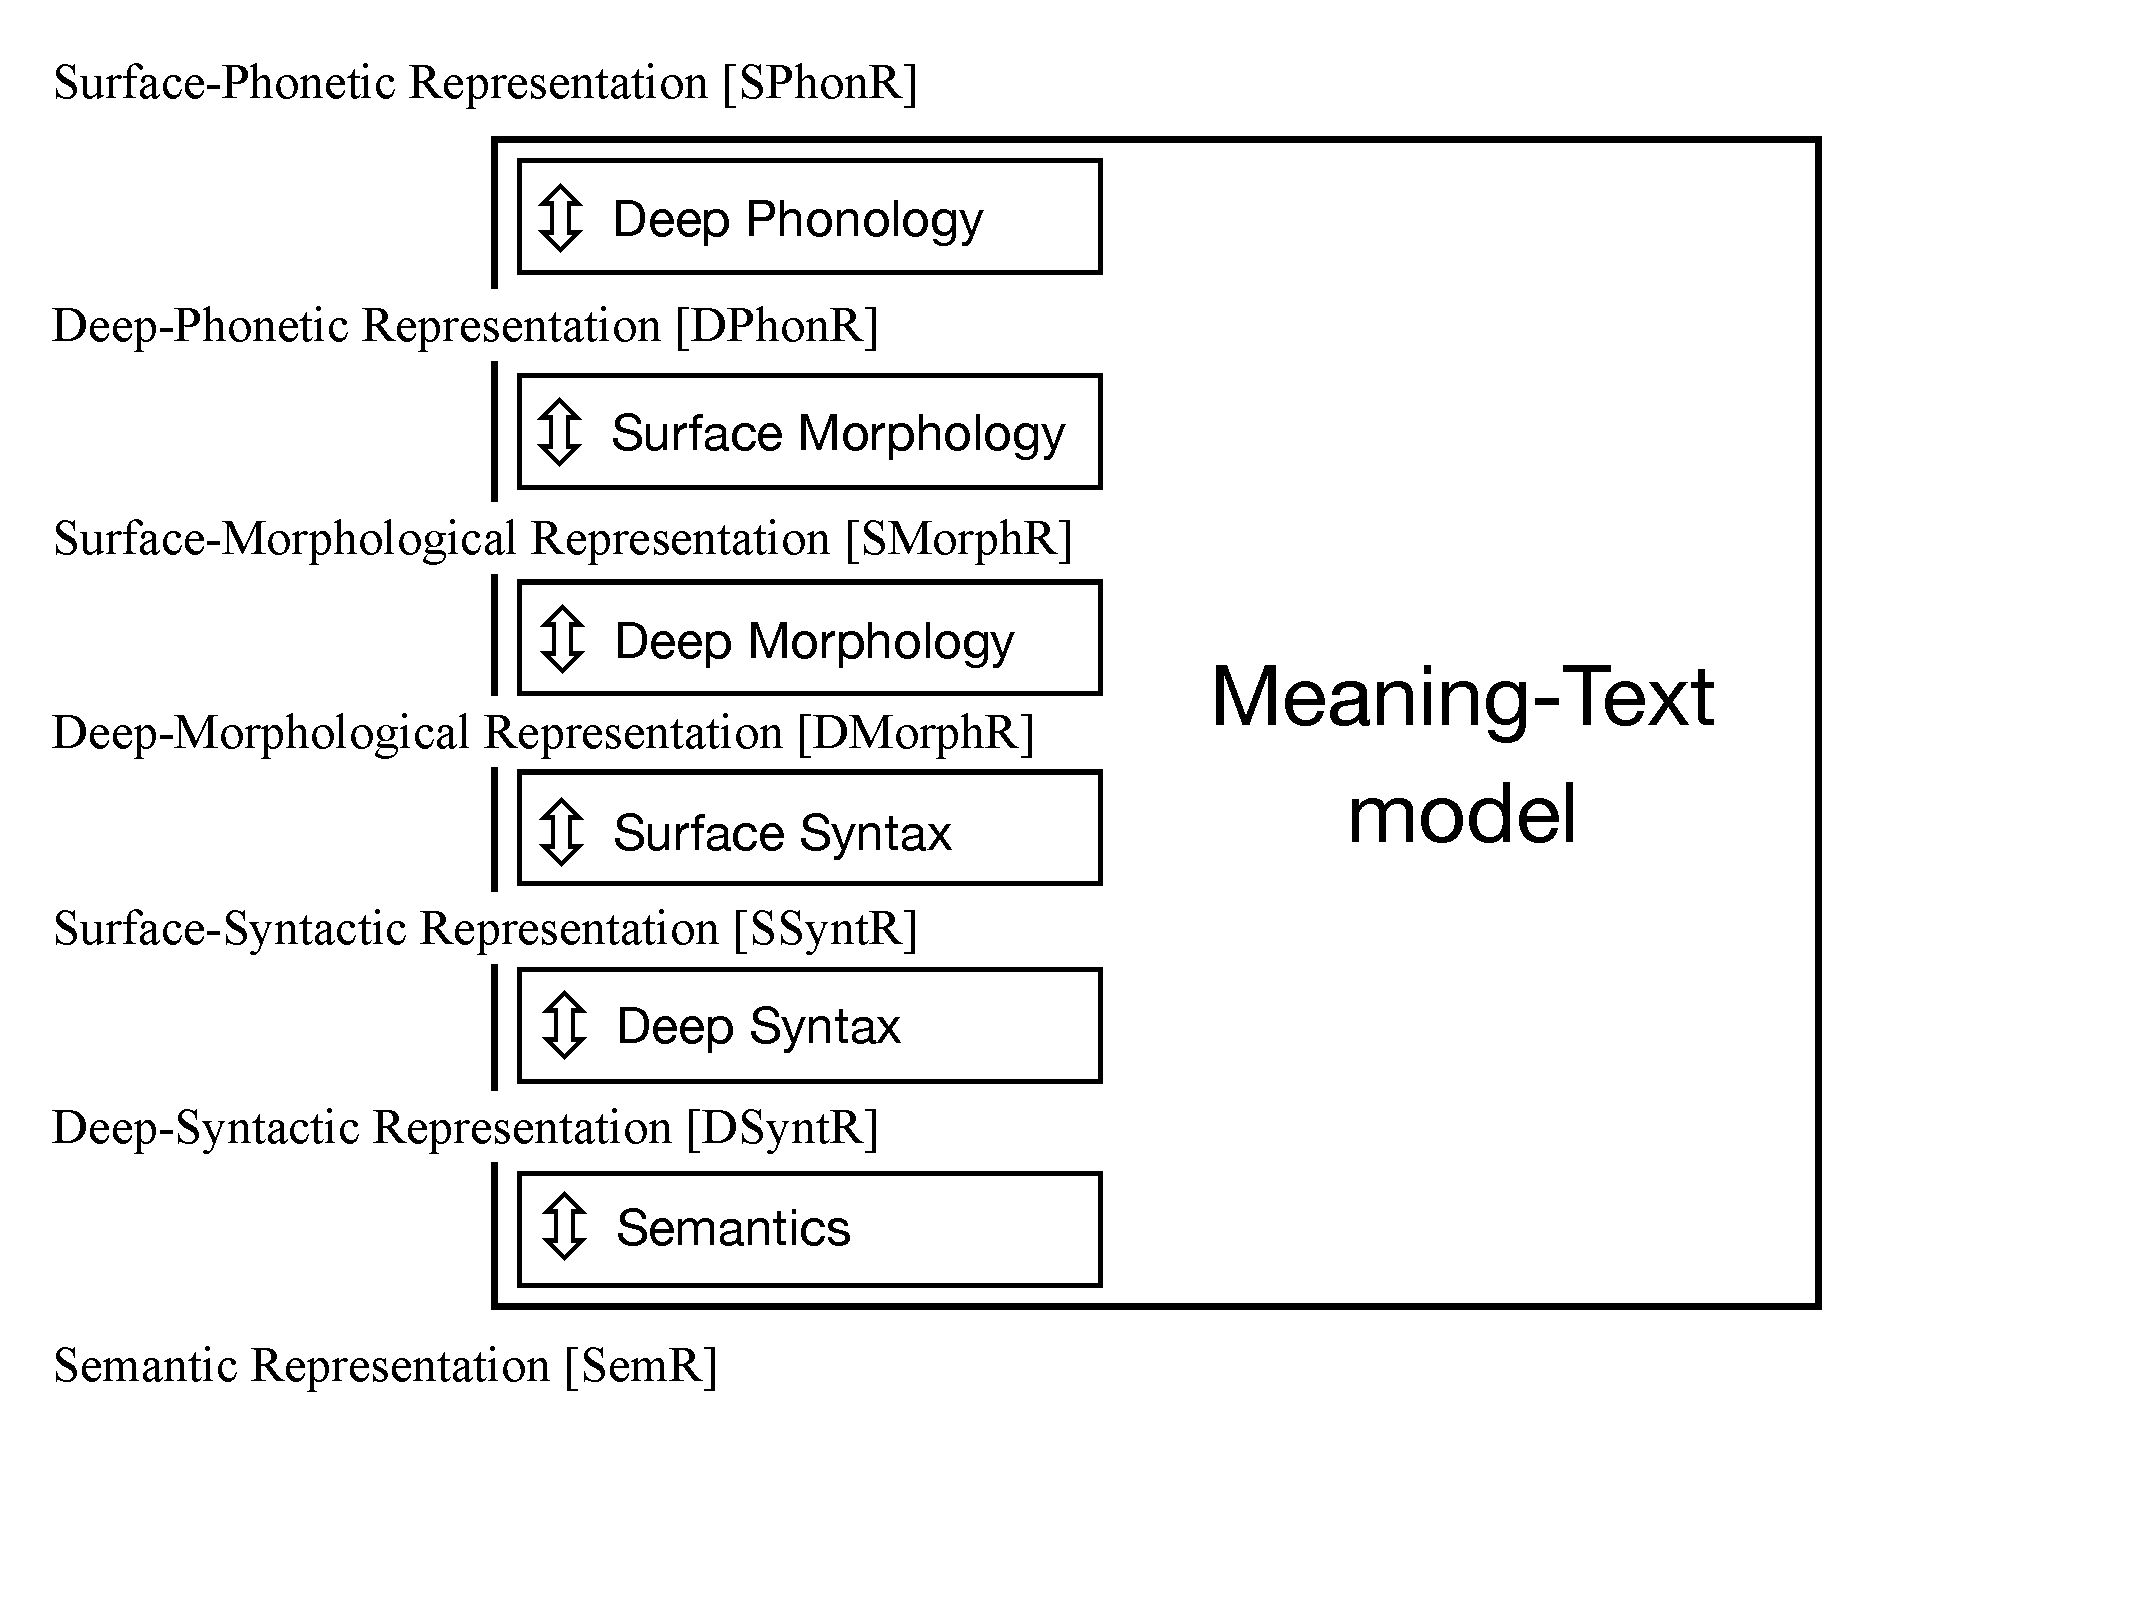
\includegraphics[width=0.8\linewidth]{Fig/Introduction/architectureMTM.pdf}
\caption{Architecture of a Meaning-Text model}\label{fig:MTTModules}
\end{figure}

Second, we have to acknowledge that the formal language of lexical functions\index[notion]{lexical function!formal language of \tlds} is far from being streamlined and self-evident. It tries to reconcile two mutually incompatible imperatives: on the one hand, formal precision; on the other hand, legibility by humans and the possibility of easily applying the researcher's linguistic intuition when reasoning on lexical function formulas. Consequently, the language of lexical functions is sometimes making use of unusual formal conventions -- for instance, the use of actantial subscripts\index[notion]{actantial subscript} (to the names of lexical functions) with different interpretations depending on the context, which is not acceptable in a genuine formal language (\chapref{chap:NotionLF}, Sections~\ref{sec:actSubsSimpleLF} and \ref{sec:actSubsLFCombinations}).\footnote{For an alternative (so-called \textit{algebraic}) notation of lexical functions, see \textcite{KahanePolguere2001-e}. Note that what is gained with this notation in terms of formal rigor and calculability is counterbalanced by a clear loss in terms of possible recourse to linguistic intuition when a lexicographer, a linguist, etc., wants to reason using lexical functions.}

Faced with these difficulties, we decided to deal with the situation frontally, without cutting corners. However, because our ambition is, first of all, to be as much pedagogical as possible, we made a systematic effort at providing readers with all background and, even, insider knowledge needed to achieve an in-depth understanding of lexical functions. We hope therefore that the book can prove useful to a vast range of readers: linguists, lexicographers, researchers and developers in Natural Language Processing, language teachers, translators, etc. -- in a nutshell, to everyone who deals with or is interested in Language.

\section{How do we describe lexical functions?}\label{sec:howDoWeDescribeLFs}

As we just said, this book is intended as a fresh, more pedagogical presentation of the system of lexical functions, which has already been the topic of many publications -- e.g., \textcite{AlonsoRamos1993}, \textcite{Melcuk1996}, \textcite{Melcuk2007b}, \textcite[210--223]{MelcukMilicevic2014a}, \textcite[Ch.~14]{Melcuk2015a-e}, etc. So  how are we proceeding to achieve this pedagogical goal?

\paragraph*{Chapter organization.}

To start with, the chapter organization follows a progression that aims at a gradual acquisition of lexical functions:

\begin{itemize}
\setlength\itemsep{0pt}

\item Chapter~\ref{chap:preliminaryNotions} introduces some basic lexicological, semantic and syntactic notions the knowledge of which is a prerequisite for the assimilation of lexical functions. The presentation of these preliminary notions encompasses important terminology and formal conventions used throughout the remainder of the book.

\item Chapter~\ref{chap:NotionLF} is an in-depth discussion of the notion of lexical function. It is intended to familiarize readers with all conceptual and formal aspects of lexical functions on which the description of individual lexical functions in the following chapters is based.

\item Chapter~\ref{chap:paraLFs} presents, in a logical order,\index[notion]{lexical function!ordering of \tlds}\index[notion]{ordering of LFs} all paradigmatic simple standard lexical functions.

\item Chapter~\ref{chap:syntLFs} does the same for syntagmatic simple standard lexical functions.

\item Chapter~\ref{chap:lexicalNetwork} concludes the book with the discussion of the central role played by lexical functions in the structuring of natural language lexicons modeled as lexical networks.

\end{itemize}

While readers are expected to study Chapters~\ref{chap:preliminaryNotions} and~\ref{chap:NotionLF} in a linear way, Chapters~\ref{chap:paraLFs} and~\ref{chap:syntLFs} are designed for random, or ``opportunistic,'' access to information on individual lexical functions. A profusion of cross-references helps establish connections between conceptually related lexical functions, thus allowing readers to browse a \emph{system}\index[notion]{lexical function!system of standard \tlds} of lexical functions, rather than following a one-way path through a \emph{list}.

\paragraph*{Detailed description template of lexical functions.}

The presentation of individual lexical functions follows a well-specified template that is explained in \chapref{chap:NotionLF}, \sectref{sec:descriptionTemplateLF}. We have paid special attention to providing information required for \emph{active} learning, where readers can not only understand what a given lexical function is, but also develop the ability to use it in various contexts (lexicographic work\index[notion]{lexicography}, language teaching\index[notion]{teaching\slashs{}learning, language}\index[notion]{language teaching\slashs{}learning}, etc.).

As the book contains updates to the system of standard lexical functions that might be confusing with respect to information and practices found in earlier publications, \textit{Historical remarks} have been added at the relevant points to help the readers in this respect.

\paragraph*{Extensive linguistic exemplification.}

Though standard lexical functions are postulated to be language-universal\index[notion]{language-universal}, it would have been a colossal task to systematically illustrate each given lexical function with examples borrowed from a broad range of typologically different language families. However, to take into consideration the cross-linguistic relevance of lexical functions, our illustrations in the presentation of lexical functions are systematically done in English, French and Russian -- the latter two being the mother tongues of the authors.

\paragraph*{Facilitation of multiple access to information.}

We did not hesitate to introduce some redundancies in the volume in order to facilitate the different types of usage by readers: in-depth learning of the nature and use of lexical functions vs. punctual consultation of the description of individual lexical functions. In the same spirit, indexes (of notions and of lexical functions) are extensive, with some form of redundancy at times, in order to meet the multiple needs of individual readers.

Note that the full list of standard lexical functions is available in two forms: as an alphabetical list (p.\thinspace\pageref{chap:listLFs}); and as a~``logical'' list (\chapref{chap:NotionLF}, p.\thinspace\pageref{tab:systFL}), where lexical functions are enumerated in the order\index[notion]{lexical function!ordering of \tlds}\index[notion]{ordering of LFs} they appear in Chapters~\ref{chap:paraLFs} and~\ref{chap:syntLFs}.

\paragraph*{Alternative approaches.}

As explained in Section~\ref{sec:aboutWhat}, lexical functions serve to describe both collocations, embodying syntagmatic lexical relations, \emph{and} derivations, embodying paradigmatic lexical relations. There exists a wealth of literature on these topics, which are generally treated as two non-related lexical phenomena; but the systematic presentation of alternative approaches to lexical functions is beyond the scope of the present book. We establish connections between the lexical function approach to the description of lexical relations and other well-known approaches when it is especially relevant to do so. In particular, current approaches to the description of collocations in lexicographic models are examined at the end of Chapter~\ref{chap:syntLFs}, on syntagmatic lexical functions (\sectref{sec:Non-LFApproachesCollocations}, p.\thinspace\pageref{sec:Non-LFApproachesCollocations}); semantic lexical relations for the structuring of so-called \textit{-Net} models\index[notion]{model!-Net@\textit{-Net} \tld}\index[notion]{net@\textit{-Net} model} (cf. WordNet\index[notion]{WordNet}\index[notion]{lexical database!WordNet}) are contrasted with the use of paradigmatic lexical functions in Chapter~\ref{chap:lexicalNetwork}, on lexical networks (\sectref{sec:shapeOfLexicons}, p.\thinspace\pageref{sec:shapeOfLexicons}).

\section*{Acknowledgments}

\textit{Lexical functions: The naked truth} exploits material from a paper (in French) entitled \textit{Les fonctions lexicales dernier cri} \parencite{MelcukPolguere2021}. We are grateful to Sébastien Marengo, the editor of the volume in which the paper was published, for the permission to make use of this text.

We have benefited from comments made by Margarita Alonso Ramos, David Beck, Alastair Butler, Lise Fontaine, Lidija Iordanskaja, Anne-Laure Jousse, Sylvain Kahane, Robert Krovetz, François Lareau, Veronika Lux-Pogodalla, \begin{otherlanguage}{french}Sébastien Marengo\end{otherlanguage}, Sandrine Ollinger, Monica Pasqualini as well as two anonymous reviewers.

The following proofreaders for Language Science Press saved us from countless blunders: Amy Amoakuh, 
Barend Beekhuizen, Anca G\^{a}\textcommabelow{t}\u{a}, Matthew Korte, César Millán, Jean Nitzke, Ikmi Nur Oktavianti,
Elliott Pearl, Valeria Quochi, Nicoletta Romeo and Mary Ann Walter.

And last but not least, our very special word of gratitude goes to Stefan Müller and Sebastian Nordhoff, who -- two wise pilots -- took our book to a safe haven.

\clearpage{\pagestyle{empty}\cleardoublepage}

